%%%%%%%%%%%%%%%%%%%%%%%%%%%%%%%%%%%%%%%%%%%%%%%%%%%%%%%%%%%%%%%%%%%%%%%%%%%%%%%%%%%%
%%%%%%%%%%%          Preamble
%%%%%%%%%%%%%%%%%%%%%%%%%%%%%%%%%%%%%%%%%%%%%%%%%%%%%%%%%%%%%%%%%%%%%%%%%%%%%%%%%%%% 
\documentclass[9pt]{beamer}
\usepackage{setspace}
\usepackage{color}
\usepackage{amsmath,lmodern}
\usepackage{hyperref}
\usepackage{graphicx}
\usepackage{multirow}
\usepackage{bm}
\usepackage{graphicx}
\usepackage{subfig}
\usepackage[textfont={scriptsize}]{caption}
\usepackage{tikz}
\usetikzlibrary{fit,shapes.misc}
\usepackage{pdflscape}
\usepackage{amsmath}
\usepackage{lscape}
\usepackage{enumerate}
\usepackage{epstopdf}
\usepackage{appendixnumberbeamer}
\usepackage{bigints}
\usepackage{booktabs}
\usepackage{color,soul}
\usepackage{grffile}
\usepackage{relsize}
% Packages
\usepackage{amsmath, amssymb, bm}
\usepackage{graphicx}
\usepackage{tikz}
\usetikzlibrary{arrows.meta, positioning}

% Colors
\definecolor{slideblue}{RGB}{0, 102, 153}
\setbeamercolor{frametitle}{fg=slideblue}
\setbeamercolor{title}{fg=slideblue}
\setbeamercolor{structure}{fg=slideblue}
\setbeamercolor{alerted text}{fg=red}

% Tighter itemize spacing
\setlength{\leftmargini}{1em}
\setlength{\leftmarginii}{1em}

% Footer
\setbeamertemplate{footline}{%
  \leavevmode%
  \hbox{%
    \begin{beamercolorbox}[wd=.33\paperwidth,ht=2.25ex,dp=1ex,left]{author in head/foot}%
      \usebeamerfont{author in head/foot}\hspace{1em}ECON712
    \end{beamercolorbox}%
    \begin{beamercolorbox}[wd=.34\paperwidth,ht=2.25ex,dp=1ex,center]{title in head/foot}%
      \usebeamerfont{title in head/foot}Winter 2026
    \end{beamercolorbox}%
    \begin{beamercolorbox}[wd=.33\paperwidth,ht=2.25ex,dp=1ex,right]{date in head/foot}%
      \usebeamerfont{date in head/foot}Lectures 14\hspace{1em}
      \insertframenumber{} / \inserttotalframenumber\hspace{1em}
    \end{beamercolorbox}}%
  \vskip0pt%
}
\newcounter{nodemarkers}
\usepackage{tikz}
\newcommand{\toplinesmall}{%
  \tikz[remember picture,overlay] {%
    \draw[blue,thick] ([yshift=-.9cm, xshift=.9cm]current page.north west)
             -- ([yshift=-.9cm,xshift=3.6cm]current page.north west);}}
             
\newcommand{\toplinemedium}{%
  \tikz[remember picture,overlay] {%
    \draw[blue,thick] ([yshift=-.9cm, xshift=.9cm]current page.north west)
             -- ([yshift=-.9cm,xshift=6.2cm]current page.north west);}}
 
 \newcommand{\toplinelarge}{%
  \tikz[remember picture,overlay] {%
    \draw[blue,thick] ([yshift=-.9cm, xshift=.9cm]current page.north west)
             -- ([yshift=-.9cm,xshift=8.9cm]current page.north west);}}           
             
 \newcommand{\toplinexlarge}{%
  \tikz[remember picture,overlay] {%
    \draw[blue,thick] ([yshift=-.9cm, xshift=.9cm]current page.north west)
             -- ([yshift=-.9cm,xshift=12cm]current page.north west);}}                       
             
\setbeamertemplate{footline}
{
  \leavevmode%
  \hbox{%
  \begin{beamercolorbox}[wd=.333333\paperwidth,ht=2.25ex,dp=1ex,center]{author in head/foot}%
    \usebeamerfont{author in head/foot}{\textcolor{blue}{ECON712}}
  \end{beamercolorbox}%
  \begin{beamercolorbox}[wd=.333333\paperwidth,ht=2.25ex,dp=1ex,center]{title in head/foot}%
    \usebeamerfont{title in head/foot}{\textcolor{blue}{Winter 2026}}
  \end{beamercolorbox}%
  \begin{beamercolorbox}[wd=.333333\paperwidth,ht=2.25ex,dp=1ex,right]{date in head/foot}%
    \usebeamerfont{date in head/foot}{\textcolor{blue}{Lectures 14 \: \: \: \: \: \: \: }
    \insertframenumber{} / \inserttotalframenumber\hspace*{2ex}} 
  \end{beamercolorbox}}%
  \vskip0pt%
}
\newtheorem{proposition}[theorem]{Proposition}

\newcommand\marktopleft[1]{%
    \tikz[overlay,remember picture] 
        \node (marker-#1-a) at (-0.2,1.2ex) {};%
}
\newcommand\markbottomright[1]{%
    \tikz[overlay,remember picture] 
        \node (marker-#1-b) at (0.16,-1ex) {};%
    \tikz[overlay,remember picture,thick,inner sep=4pt]
        \node[draw,rectangle,rounded corners, blue, fit=(marker-#1-a.center) (marker-#1-b.center)] {};%
}

\setbeamertemplate{itemize items}[ball]
\setbeamertemplate{itemize subitem}[triangle]
\setbeamertemplate{itemize subsubitem}[triangle]
\beamertemplatenavigationsymbolsempty
\addtobeamertemplate{frametitle}{\vspace*{0.19cm}}{\vspace*{0cm}}



%%%%%%%%%%%%%%%%%%%%%%%%%%%%%%%%%%%%%%%%%%%%%%%%%%%%%%%%%%%%%%%%%%%%%%%
%%%%%%%%%%%%%%%%%%%%%%%%%%%%%%%%%%%%%%%%%%%%%%%%%%%%%%%%%%%%%%%%%%%%%%% 
%%%%%%%%%  									    Define Title									                                       %%%%%%%%%
%%%%%%%%%%%%%%%%%%%%%%%%%%%%%%%%%%%%%%%%%%%%%%%%%%%%%%%%%%%%%%%%%%%%%%%
%%%%%%%%%%%%%%%%%%%%%%%%%%%%%%%%%%%%%%%%%%%%%%%%%%%%%%%%%%%%%%%%%%%%%%% 
\title{ECON 712: Applied Econometrics} 
\author{Lecture 14: Instrumental Variables}
\date{}
\AtBeginSection[]
{
 \begin{frame}<beamer>
 \tableofcontents[currentsection]
 \end{frame}
}



%%%%%%%%%%%%%%%%%%%%%%%%%%%%%%%%%%%%%%%%%%%%%%%%%%%%%%%%%%%%%%%%%%%%%%%
%%%%%%%%%%%%%%%%%%%%%%%%%%%%%%%%%%%%%%%%%%%%%%%%%%%%%%%%%%%%%%%%%%%%%%% 
%%%%%%%% 						     				Document								                                                %%%%%%%%
%%%%%%%%%%%%%%%%%%%%%%%%%%%%%%%%%%%%%%%%%%%%%%%%%%%%%%%%%%%%%%%%%%%%%%%
%%%%%%%%%%%%%%%%%%%%%%%%%%%%%%%%%%%%%%%%%%%%%%%%%%%%%%%%%%%%%%%%%%%%%%% 
\begin{document}
\setbeamercovered{transparent}


\begin{frame}
\maketitle
\end{frame}

\section{Instrumental Variables}

\begin{frame}
\frametitle{\: \: \: Instrumental Variables}
\toplinemedium
\begin{itemize}
\item There are instances that we cannot solve issues endogeneity by adding controls, e.g.
\begin{itemize}
\vspace{0.11in}
\item Omitted variable bias: the omitted variable is not observed
\vspace{0.11in}
\item Treatment Effects: the treatment assignment does not satisfy the CIA assumption for any set of observable covariates
\end{itemize}
\vspace{0.11in}
\item In this case, we can solve the issue by finding an instrument, $Z$, that allows us to identify the casual effect of an endogenous variable, $X$
\begin{itemize}
\vspace{0.11in}
\item An instrument is a variable that only affects the outcome variable through $X$ and that does not correlates with unobserved variables affecting the outcome variable
\end{itemize}
\end{itemize}
\end{frame} 

\begin{frame}
\frametitle{\: \: \: E.g. Ommitted variable bias}
\toplinemedium
Suppose the true causal model is:
  \begin{center}
  \begin{tikzpicture}[node distance=1.5cm, every node/.style={font=\small},
                      arr/.style={-{Stealth}, thick}]
    \node (eps) {$\varepsilon$};
    \node (X) [below left=1.0cm and 0.7cm of eps] {$X$};
    \node (Y) [below right=1.0cm and 0.7cm of eps] {$Y$};
    \node (A) [below=1.2cm of X, xshift=0.7cm] {$A$};
    \draw[arr] (eps)--(Y); \draw[arr] (X)--(Y);
    \draw[arr] (A)--(X);   \draw[arr] (A)--(Y);
  \end{tikzpicture}
  \end{center}
This gives: $y = \beta_0 + \delta x + \beta_1 A + \epsilon$
 
  \medskip
  \begin{itemize}
    \item An instrument $z$ satisfies:
  \end{itemize}
  \begin{center}
  \begin{tikzpicture}[node distance=1.5cm, every node/.style={font=\small},
                      arr/.style={-{Stealth}, thick}]
    \node (eps) {$\varepsilon$};
    \node (X) [below=1.0cm of eps, xshift=-0.3cm] {$X$};
    \node (Y) [right=2.0cm of X] {$Y$};
    \node (Z) [left=1.8cm of X] {$Z$};
    \node (A) [below=1.0cm of X, xshift=0.7cm] {$A$};
    \draw[arr] (eps)--(Y); \draw[arr] (Z)--(X);
    \draw[arr] (X)--(Y);   \draw[arr] (A)--(X); \draw[arr] (A)--(Y);
  \end{tikzpicture}
  \end{center}
\end{frame}

\begin{frame}
\frametitle{\: \: \: E.g. Omitted variable bias}
\toplinemedium
\begin{itemize}
\item In this case, if we estimate the relation: $y=\beta_0+\delta \: x+\eta$, where   $\eta=\beta_2 \: A+\epsilon$ using a sample an applying OLS to solve for $\hat{\delta}$, we would get a biased and inconsistent estimator
\vspace{0.11in}
\item However, note that: i. $Cov(z,x) \neq 0$, ii. $Cov(z,\eta)=0$ (due to $E[\eta|z]=0$--- \textcolor{blue}{exclusion restriction}), and iii. $z$ only affects $y$ through x
\begin{itemize}
\vspace{0.11in}
\item Question: If we observe $z$, can we use this variable to help us estimate $\delta$? The answer is \textcolor{blue}{YES}
\end{itemize} 
\vspace{0.11in}
\item In the case that we do not observe $A$, but we have a variable $z$, we could use the following relationship:
\begin{eqnarray*}
\delta=\frac{Cov(y,z)}{Cov(x,z)}=\frac{\gamma_1}{\alpha_1}
\end{eqnarray*}
where:
\begin{eqnarray*}
\begin{array}{lll}
y=\gamma_0+\gamma_1 \: z+u &E[u|z]=E[u]=0 & \text{Reduced-Form} \\ 
x=\alpha_0+\alpha_1 \: z+\nu &E[\nu|z]=E[\nu]=0 & \text{First-Stage} \\
\end{array}
\end{eqnarray*}
\end{itemize}
\end{frame}

\begin{frame}
\frametitle{\: \: \: IV Estimate}
\toplinemedium
\begin{itemize}
\item Using a sample to estimate parameters:
\begin{eqnarray*}
\begin{array}{lll}
\hat{\delta}^{IV}=\frac{\hat{\gamma}_1}{\hat{\alpha}_1} &,  \hat{\gamma}_1=\frac{\mathlarger{\sum}_{i=1}^{n}(y_i-\overline{y})(z_i-\overline{z})}{\mathlarger{\sum}_{i=1}^{n}(z_i-\overline{z})^2} &,  \hat{\alpha}_1=\frac{\mathlarger{\sum}_{i=1}^{n}(x_i-\overline{x})(z_i-\overline{z})}{\mathlarger{\sum}_{i=1}^{n}(z_i-\overline{z})^2} 
\end{array}
\end{eqnarray*}
\item We cannot show unbiasedness in finite samples, but we can show:
\begin{eqnarray*}
plim(\hat{\delta}^{IV}-\delta)=\frac{plim \: \mathlarger{\sum}_{i=1}^{n}(z_i-\overline{z}) \: \eta}{plim \: \mathlarger{\sum}_{i=1}^{n}(x_i-\overline{x})(z_i-\overline{z}) }=\frac{Corr(z,\eta) \: \sigma_{\eta}}{Corr(x,z) \: \sigma_x}=0
\end{eqnarray*}
\end{itemize}
\end{frame}

\begin{frame}
\frametitle{\: \: \: \textcolor{blue}{2SLS}}
\toplinesmall
\begin{itemize}
\item In practice, we use a the following procedure called 2SLS (e.g. with one endogenous variable and one instrument) 
\begin{eqnarray*}
\begin{array}{lll}
y_i=\bm{W_i}^T \bm{\beta}+\delta \: \hat{x}_i+ \xi_i  &, &  E[\xi|\bm{W_i}, \hat{x}]=0
\end{array}
\end{eqnarray*}
\begin{itemize}
\item Where $\hat{x}_i=\bm{W_i}^T \bm{\pi}+\alpha z_i$ and $\xi=\eta_i+\delta \nu_i$
\vspace{0.11in}
\item Also, $E[\eta|z]=E[\eta]$ (by exclusion restriction), $E[\nu|z]=E[\nu]$ (by first stage) 
\vspace{0.11in}
\end{itemize}
\item That is $\delta$ is estimated from the variation of $x$ that is due to $z$ only
\end{itemize}
\end{frame}


\begin{frame}
\frametitle{\: \: \: \textcolor{blue}{2SLS} in practice}
\toplinemedium
\begin{itemize}
\item In practice:
\begin{enumerate}
\item Estimate $\bm{\pi}$, $\alpha$ from the first stage using OLS and obtain:
\begin{eqnarray*}
\hat{x}_i=E[x|z_i]=\bm{W_i}^T \bm{\hat{\pi}}+\hat{\alpha} \: z_i
\end{eqnarray*}
\item Substitute this into main equation and estimate $\bm{\beta}$ and $\delta$ using OLS:
\begin{eqnarray*}
\begin{array}{lll}
y_i=\bm{W_i}^T \bm{\hat{\beta}}^{2sls}+\hat{\delta}^{2sls} \: \hat{x}_i+ \hat\xi_i &,& \hat\xi_i=\hat{\eta}_i+\hat{\delta} (x_i-\hat{x}_i)
\end{array}
\end{eqnarray*}
\end{enumerate}
\item In the case of one endogenous variable and one instrument this estimator is the same as the one presented above:
\begin{eqnarray*}
\hat{\delta}^{2sls}=\frac{(\bm{M_w \: z})^T \bm{y}}{(\bm{M_w \: z})^T (\bm{M_w \: z})}\frac{1}{\hat{\alpha}}=\hat{\delta}^{IV}
\end{eqnarray*}
\vspace{0.11in}
\item Standard errors for $\hat{\delta}^{2sls}$ are larger than on the OLS case due to:
\begin{enumerate}
\vspace{0.11in}
\item Variation in  $\hat{x}$ is a subset of variation in $x$
\vspace{0.11in}
\item The uncertainty from the first stage estimation needs to be accounted for
\end{enumerate}
\end{itemize}
\end{frame}

\begin{frame}
\frametitle{\: \: \: \textcolor{blue}{2SLS}: General Case}
\toplinemedium
\begin{itemize}
\item Suppose you have the following model:
\begin{eqnarray*}
y_i=\beta_0+\beta_1 x_i+\beta_2\ w_{1i} +\cdots+\beta_{k+1} w_{ki}+\eta_i
\end{eqnarray*}
\item Assume that $x$ is endogenous but that you have $j$ instruments, then:
\begin{itemize}
\vspace{0.11in}
\item From the first stage you get:
\begin{eqnarray*}
\hat{x}_i=\hat{\alpha}_0+\hat{\alpha}_0\ w_{1i} +\cdots+\hat{\alpha}_k w_{ki}+\hat{\alpha}_{k+1} z_{1i}+\cdots+\hat{\alpha}_{k+j} z_{ji}
\end{eqnarray*}
\item The substitute this for $x_i$ into the estimating equation and estimate coefficients:
\begin{eqnarray*}
y_i=\hat{\beta}_0+\hat{\beta}_1 \hat{x}_i+\hat{\beta}_2\ w_{1i} +\cdots+\hat{\beta}_{k+1} w_{ki}+\hat{\xi}_i
\end{eqnarray*}
\end{itemize}
\item There could also be multiple endogenous variables as well, in which case we need to write it in vector form
\end{itemize}
\end{frame} 

\begin{frame}
\frametitle{\: \: \: \textcolor{blue}{2SLS}: General Vector Form}
\toplinemedium

 \textbf{Setup.} Partition regressors into exogenous controls $\mathbf{W}$ ($n\times k_1$)
and endogenous variables $\mathbf{X}_{\!2}$ ($n\times k_2$):
\[
  \mathbf{y} = \mathbf{W}\bm{\alpha} + \mathbf{X}_{\!2}\bm{\delta} + \bm{\eta}
  \;\equiv\; \mathbf{X}\bm{\beta} + \bm{\eta},
  \qquad
  \mathbf{X} = [\,\mathbf{W}\;\;\mathbf{X}_{\!2}\,] \in \mathbb{R}^{n\times(k_1+k_2)}
\]
Stack exogenous controls and $j$ excluded instruments into the instrument matrix:
\[
  \mathbf{Z} = [\,\mathbf{W}\;\;\mathbf{Z}_{\!2}\,] \in \mathbb{R}^{n\times(k_1+j)}
\]

\medskip
\textbf{Order condition (necessary for identification):}
\begin{itemize}
  \item $j = k_2$: \textcolor{blue}{just-identified} \quad
        $j > k_2$: overidentified \quad
        \alert{$j < k_2$: underidentified ---
        \textbf{cannot estimate} $\bm{\delta}$}
\end{itemize}

\medskip
\textbf{2SLS estimator.}
Let $\mathbf{P}_Z = \mathbf{Z}(\mathbf{Z}^\top\mathbf{Z})^{-1}\mathbf{Z}^\top$:
\[
  \boxed{
    \hat{\bm{\beta}}^{2SLS}
    = \bigl(\mathbf{X}^\top \mathbf{P}_Z \mathbf{X}\bigr)^{-1}
      \mathbf{X}^\top \mathbf{P}_Z\,\mathbf{y}
  }
\]
Intuitively, $\mathbf{P}_Z\mathbf{X}$ purges $\mathbf{X}_{\!2}$ of its endogenous component,
keeping only the variation attributable to $\mathbf{Z}$.

\end{frame}


\begin{frame}
\frametitle{\: \: \: \textcolor{blue}{2SLS}: Asymptotic Distribution}
\toplinemedium
We can derive the asymptotic distribution of the \textbf{2SLS} estimator as follows:
\[
\sqrt{n}(\hat{\bm{\beta}}^{2sls}-\bm{\beta})
\xrightarrow{d}
N\!\left(
\bm{0},
S_{V^{\top}V}^{-1}
\mathbb{E}\left[\bm{V}_i \eta_i^2 \bm{V}_i^T\right]
S_{V^{\top}V}^{-1}
\right)
\]
\begin{itemize}
    \item where $P_z \bm{X}=V\left[\bm{W} \  \mathbf{\hat{X}}_{\!2}\right]$  % fixed: \right] not \right$
\end{itemize}
\vspace{0.11in}
As in the case of OLS:
\begin{itemize}
\vspace{0.11in}
    \item For homoscedastic error terms we estimate the variance as:
    \begin{eqnarray*}
    \begin{array}{lll}
    Var(\bm{\hat{\beta}}^{2sls})=\hat{\sigma}^2_{\eta} (\bm{V}^T \bm{V})^{-1} &,& \hat{\sigma}^2_{\eta}=(n-k)^{-1}\bm{\hat{\eta}}^T \bm{\hat{\eta}}
    \end{array}
    \end{eqnarray*}
\vspace{0.11in}
    \item For heteroscedastic error terms, we use the sandwich estimator:
    \begin{eqnarray*}
    (\bm{V}^T \bm{V})^{-1} \bm{V}^T \bm{\hat{\Sigma}_{\eta}} \bm{V} (\bm{V}^T \bm{V})^{-1}
    \end{eqnarray*}
\end{itemize}
\end{frame}

\begin{frame}
\frametitle{\: \: \: \textcolor{blue}{2SLS}: Asymptotic Distribution}
\toplinemedium
There are \textbf{two} important considerations:
\begin{enumerate}
    \item Residual used in estimating the variance of the error term is:
    \begin{eqnarray*}
        \hat{\eta}_i=y_i-\bm{X}^T \bm{\hat{\beta}}^{2sls}
    \end{eqnarray*}
    and \textcolor{red}{not} the residual of the second stage:
    \begin{eqnarray*}
        \hat{\eta}_i+(\bm{X}_i-\bm{\hat{X}}_i)^T \bm{\hat{\beta}}^{2sls}=y_i-\bm{\hat{X}}^T(\bm{\hat{\beta}}^{2sls})  % fixed: \( -> (
    \end{eqnarray*}
    \begin{itemize}
        \item That is implementing 2SLS manually uses the wrong residuals. Use \texttt{ivreg} or \texttt{ivreg2} in STATA to calculate the correct standard errors (similar command in R)
    \end{itemize}
   \vspace{0.11in}
    \item Elements of $(\bm{V}^T \bm{V})^{-1}$ are hard to analyze, but we know that:
     \[\bm{V}^T \bm{V}=\bm{X}^T P_z \bm{X}\]
    \begin{itemize}
        \item Main diagonal are the result of vector multiplication, therefore, if instruments are weakly correlated with the endogenous variables these elements go to zero
        \vspace{0.11in}
        \item Weak instruments result in large variances because the first stage is not estimated precisely
    \end{itemize}
\end{enumerate}
\end{frame}


\begin{frame} \label{IV}
\frametitle{\: \: \: \textcolor{blue}{2SLS}: Further Considerations}
\toplinemedium
\begin{enumerate}
\item The problem of \textcolor{red}{weak} instruments is not only a problem for the SE but it also results in biased 2SLS estimates even in LARGE SAMPLES!!!
\begin{itemize}
\vspace{0.11in}
\item To check for weak instruments we run an F-test of excluded instruments on the first stage (with multiple endogenous variables, we run multiple F-Tests)
\hyperlink{Ftest}{\beamerbutton{F Test}}
\end{itemize}
\vspace{0.11in}
\item 2SLS only works with linear instruments because the estimated endogenous variable inherits the exclusion restriction property \textbf{only} when the first stage is linear
\begin{itemize}
\vspace{0.11in}
\item This means that if the endogenous variable is binary, the first stage must be a LPM (running a Logit or Probit first stage is called the \textcolor{red}{forbidden} regression)
\end{itemize}

\vspace{0.11in}
\item The \textcolor{blue}{exclusion restriction} cannot be directly tested as error terms of the main regression are not observed, however, with \textcolor{red} {more} instruments than endogenous variables a test of overidentifying restrictions can be performed.
\vspace{0.11in}
\begin{itemize}
\item This tests for the validity of the instruments included in the IV estimate
\end{itemize}
\end{enumerate}
\end{frame}

\begin{frame}
\frametitle{\: \: \: IV Example: Angrist and Krueger (1991)}
\toplinelarge
\begin{itemize}
\item To resolve issues with endogeneity when measuring the returns to education,  Angrist and Krueger (1991) instrumented the years of schooling with the quarter of birth
\vspace{0.11in}
\item The idea is that if students leave school at a particular age, as in over much of the twentieth century, then students whose birthday is in the first quarter will receive less education than students in later quarters:
\begin{figure}
\centering
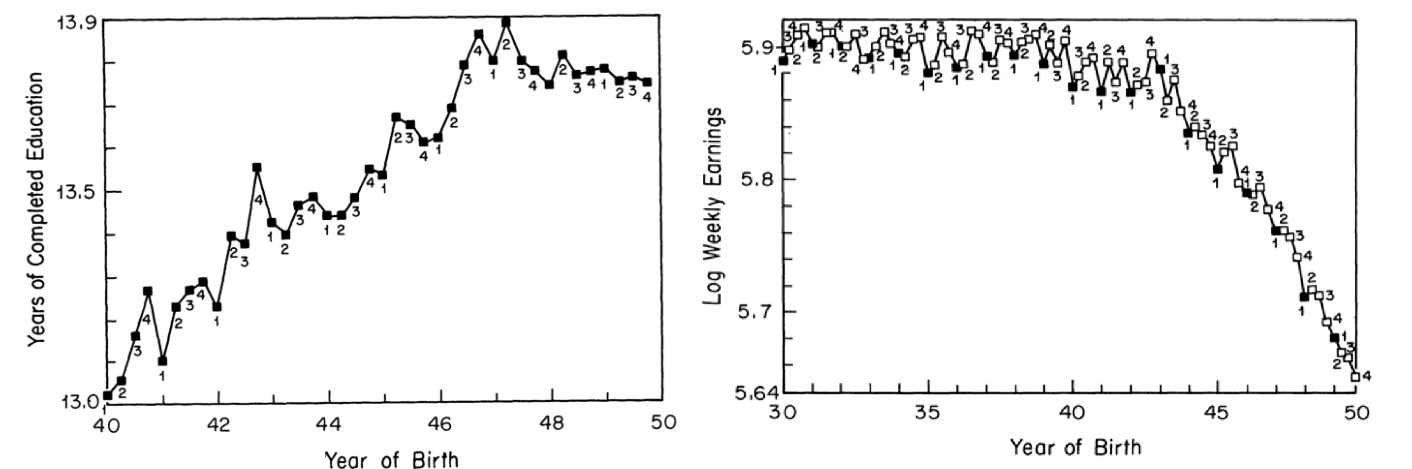
\includegraphics[scale=.29]{years_of_education}
\end{figure} 
\end{itemize}
\end{frame}


\begin{frame}
\frametitle{\: \: \: IV Example: Angrist and Krueger (1991)}
\toplinelarge
\begin{figure}
\centering
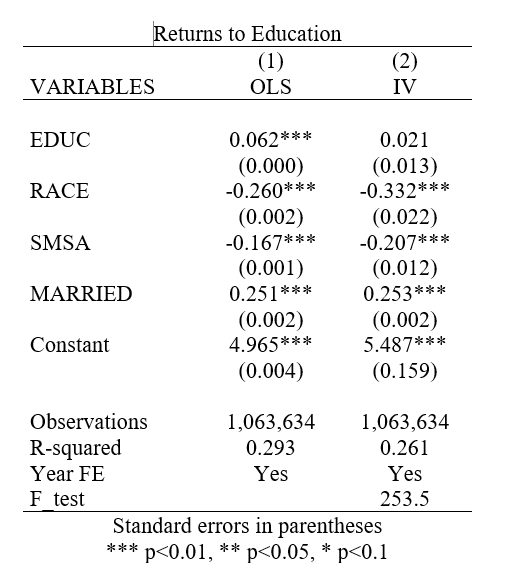
\includegraphics[scale=.45]{returns_education}
\caption*{\textbf{Note:} The dependent variable is the log weekly earnings and IV variable is $QOB$}
\end{figure} 
\end{frame}


\begin{frame}
\frametitle{\: \: \: IV Example: Angrist and Krueger (1991)}
\toplinelarge
\begin{figure}
\centering
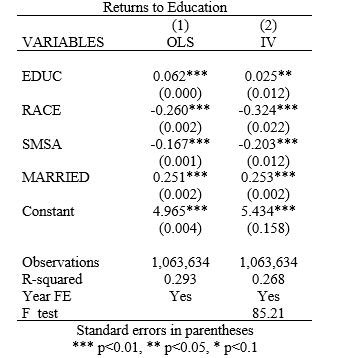
\includegraphics[scale=1]{years_of_education1}
\caption*{\textbf{Note:} The dependent variable is the log weekly earnings and IV variables are dummies for quarter 2, 3,4 of birth}
\end{figure} 
\end{frame}

\section{Instrumental Variables and Heterogeneity}

\begin{frame}
\frametitle{\: \: \: Limitations of the Constant-Effects Model}
\toplinexlarge
\begin{itemize}
\item So far we assumed: $y_i = \alpha + \delta D_i + \eta_i$, where $\delta$ is the \textbf{same} for everyone
\vspace{0.11in}
\item This rules out that individuals respond differently to treatment --- a strong assumption
\vspace{0.11in}
\item In reality, treatment effects are \textcolor{blue}{heterogeneous}:
\begin{itemize}
\vspace{0.08in}
\item Education raises wages more for some people than others
\vspace{0.08in}
\item Military service affects earnings differently across individuals
\vspace{0.08in}
\item Health insurance has different effects on different patients
\end{itemize}
\vspace{0.11in}
\item With heterogeneous effects, \textbf{which} average treatment effect does IV estimate?
\vspace{0.11in}
\item Answer (Imbens \& Angrist, 1994): the \textcolor{blue}{Local Average Treatment Effect (LATE)} --- the average effect \textit{for the subpopulation whose treatment status is changed by the instrument}
\end{itemize}
\end{frame}

\begin{frame}
\frametitle{\: \: \: Potential Outcomes Framework}
\toplinelarge
\begin{itemize}
\item Each individual $i$ has two \textcolor{blue}{potential outcomes}:
\begin{eqnarray*}
\begin{array}{ll}
Y_{1i} & \text{outcome if treated } (D_i=1) \\
Y_{0i} & \text{outcome if not treated } (D_i=0)
\end{array}
\end{eqnarray*}
\item The \textbf{observed} outcome is:
\begin{eqnarray*}
Y_i = Y_{0i} + (Y_{1i} - Y_{0i}) D_i
\end{eqnarray*}
\item The causal \textcolor{blue}{individual treatment effect} is $\delta_i = Y_{1i} - Y_{0i}$:

\item Key estimands:
\begin{eqnarray*}
\begin{array}{lll}
\text{ATE}  &=& E[Y_{1i} - Y_{0i}] \\[4pt]
\text{ATT}  &=& E[Y_{1i}-Y_{0i}\mid D_i=1] \\[4pt]
\text{LATE} &=& E[Y_{1i}-Y_{0i} \mid \text{complier}] \quad \text{(defined below)}
\end{array}
\end{eqnarray*}
\item The \textbf{fundamental problem of causal inference}: we never observe both $Y_{1i}$ and $Y_{0i}$ for the same person
\end{itemize}
\end{frame}


\begin{frame}
\frametitle{\: \: \: Introducing the Instrument}
\toplinelarge
\begin{itemize}
\item Let $Z_i \in \{0,1\}$ be a binary instrument that \textbf{encourages} treatment but does not determine it
\vspace{0.11in}
\item Define \textcolor{blue}{potential treatment} as a function of the instrument:
\begin{eqnarray*}
\begin{array}{ll}
D_{1i} & \text{treatment status of } i \text{ if } Z_i = 1 \\
D_{0i} & \text{treatment status of } i \text{ if } Z_i = 0
\end{array}
\end{eqnarray*}
\item The \textbf{observed} treatment is:
\begin{eqnarray*}
D_i = D_{0i} + (D_{1i} - D_{0i})Z_i
\end{eqnarray*}
\item Similarly define potential outcomes indexed by both treatment $d$ and instrument $z$:
\begin{eqnarray*}
Y_i(d,z) \quad d \in \{0,1\},\; z \in \{0,1\}
\end{eqnarray*}

\end{itemize}
\end{frame}


\begin{frame}
\frametitle{\: \: \: Assumptions about the instrument}
\toplinemedium
\begin{enumerate}
\item We assume that $E[\eta_i|z_i]=E[\eta_i]$, which requires that the following two components are satisfied:
\begin{itemize}
\vspace{0.11in}
\item \textcolor{blue}{Exclusion restriction} (i.e. the instrument has no direct effect): 
\begin{eqnarray*}
Y_i(1,1)=Y_i(1,0) \equiv Y_{1i} \\
Y_i(0,1)=Y_i(0,0) \equiv Y_{0i} 
\end{eqnarray*}
\item The instrument is \textcolor{blue}{as good as random}:
\begin{eqnarray*}
\{Y_i(D_{1i},1),\; Y_i(D_{0i},0),\; D_{0i},\; D_{1i}\} \;\perp\!\!\!\perp\; Z_i 
\end{eqnarray*}
\end{itemize}
\item \textcolor{blue}{First Stage (Relevance):}
\begin{eqnarray*}
E[D_{1i} - D_{0i}] \neq 0 \quad \Longleftrightarrow \quad E[D_i \mid Z_i = 1] \neq E[D_i \mid Z_i = 0] 
\end{eqnarray*}
\item \textcolor{blue}{Monotonicity (No Defiers):}
\begin{eqnarray*}
D_{1i} \geq D_{0i} \quad \text{for all } i
\end{eqnarray*}
\begin{itemize}
\item The instrument weakly \textbf{increases} everyone's probability of treatment --- no one is discouraged from treatment by a higher $Z_i$
\vspace{0.11in}
\item Rules out \textbf{defiers}: individuals who do the opposite of what the instrument encourages
\end{itemize}
\end{enumerate}
\end{frame}




\begin{frame}
\frametitle{\: \: \: The LATE Theorem }
\toplinelarge
\begin{proposition}[LATE Theorem]
Under independence, exclusion restriction, first stage, and monotonicity:
\begin{eqnarray*}
\frac{E[Y_i \mid Z_i=1]-E[Y_i \mid Z_i=0]}{E[D_i \mid Z_i=1]-E[D_i \mid Z_i=0]}
= E\!\left[\,Y_{1i}-Y_{0i}\;\big|\; D_{1i}>D_{0i}\,\right]
\end{eqnarray*}
\end{proposition}
\vspace{0.1in}
\begin{itemize}
\item The left-hand side is the \textbf{Wald estimator} --- the IV ratio with a binary instrument
\vspace{0.11in}
\item The right-hand side is the \textcolor{blue}{Local Average Treatment Effect}: the average causal effect \textbf{for compliers}
\vspace{0.11in}
\item IV does \textbf{not} identify ATE or ATT in general --- only LATE
\vspace{0.11in}
\item The word ``local'' means the estimate is local to the complier subpopulation \textit{defined by this instrument} --- it changes with the instrument
\end{itemize}
\end{frame}

\begin{frame}
\frametitle{\: \: \: Proof of LATE --- Numerator}
\toplinemedium
\textbf{Step 1 --- Reduced Form (Numerator):}
\begin{eqnarray*}
E[Y_i \mid Z_i=1] - E[Y_i \mid Z_i=0]
\end{eqnarray*}
By \textbf{exclusion restriction}:
\begin{eqnarray*}
= E\bigl[Y_{0i}+(Y_{1i}-Y_{0i})D_{i}|Z_i=1\bigr] - E\bigl[Y_{0i}+(Y_{1i}-Y_{0i})D_{i}|Z_i=0\bigr]
\end{eqnarray*}
By \textbf{independence} ($Z_i \perp (Y_{0i},Y_{1i},D_{0i},D_{1i})$), this simplifies to:
\begin{eqnarray*}
=E\bigl[Y_{0i}+(Y_{1i}-Y_{0i})D_{1i}\bigr]- E\bigl[(Y_{1i}-Y_{0i})(D_{1i}-D_{0i})\bigr]
\end{eqnarray*}
By \textbf{monotonicity} ($D_{1i}-D_{0i} \geq 0$) and the law of total expectation:
\begin{eqnarray*}
= E[\delta_i \mid D_{1i}>D_{0i}] \cdot P(D_{1i}>D_{0i})
\end{eqnarray*}

\vspace{0.05in}
\textbf{Step 2 --- First Stage (Denominator):}
\begin{eqnarray*}
E[D_i \mid Z_i=1]-E[D_i \mid Z_i=0] \stackrel{\text{indep}}{=} E[D_{1i}]-E[D_{0i}] \stackrel{\text{mono}}{=} P(D_{1i}>D_{0i})
\end{eqnarray*}
\end{frame}

\begin{frame}
\frametitle{\: \: \: Proof of LATE --- Conclusion}
\toplinemedium
\textbf{Step 3 --- Taking the Ratio:}
\begin{eqnarray*}
\frac{E[Y_i \mid Z_i=1]-E[Y_i \mid Z_i=0]}{E[D_i \mid Z_i=1]-E[D_i \mid Z_i=0]}
= \frac{E[Y_{1i}-Y_{0i} \mid D_{1i}>D_{0i}] \cdot P(D_{1i}>D_{0i})}{P(D_{1i}>D_{0i})}\\[8pt]
= E[\delta_i \mid D_{1i}>D_{0i}] \quad \blacksquare
\end{eqnarray*}
\end{frame}

\appendix

\section{Appendix}


\begin{frame}
\frametitle{\: \: \: F--Test of Excluded Instruments} \label{Ftest}
\toplinemedium
\begin{itemize}
\item To perform an F-test of excluded instruments, we need to run the following two first-stage regressions:
\begin{enumerate}
\item Unrestricted:
\begin{eqnarray*}
x_i=\hat{\alpha}_0+\hat{\alpha}_0\ w_{1i} +\cdots+\hat{\alpha}_k w_{ki}+\hat{\alpha}_{k+1} z_{1i}+\cdots+\hat{\alpha}_{k+j} z_{ji}+\hat{\epsilon}^{ur}_i
\end{eqnarray*}
\item Restricted: 
\begin{eqnarray*}
x_i=\hat{\alpha}_0+\hat{\alpha}_0\ w_{1i} +\cdots+\hat{\alpha}_k w_{ki}+\hat{\epsilon}^{r}_i
\end{eqnarray*}
\end{enumerate}
\item From these two regressions, we obtain:
\begin{eqnarray*}
\begin{array}{lr}
SSR^{ur}=\mathlarger{\sum}_{i=1}^{n} \left(\hat{\epsilon}^{ur}_i\right)^2   & SSR^{r}=\mathlarger{\sum}_{i=1}^{n}  \left(\hat{\epsilon}^{r}_i\right)^2
\end{array}
\end{eqnarray*}
\item The F-Test tests the following hypothesis:
\begin{eqnarray*}
\begin{array}{lr}
H_0: \alpha_{k+1}=\alpha_{k+2}=\cdots=\alpha_{k+j}=0 & H_A=\text{Not all coefficients are zero}
\end{array}
\end{eqnarray*}
\end{itemize}
\end{frame}



\begin{frame}
\frametitle{\: \: \: F--Test of Excluded Instruments}
\toplinemedium
\begin{itemize}
\item The F-score is calculated as follows
\begin{figure}
\centering
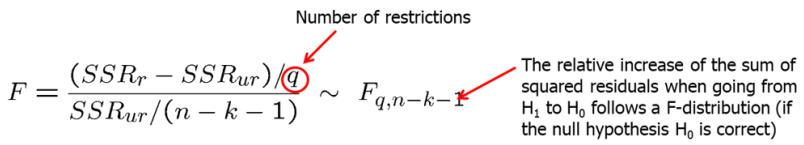
\includegraphics[scale=.4]{f_test}
\end{figure} 
\item In general, we use the F-Distribution with the appropriate level of significance to test for the Null:
\begin{figure}
\centering
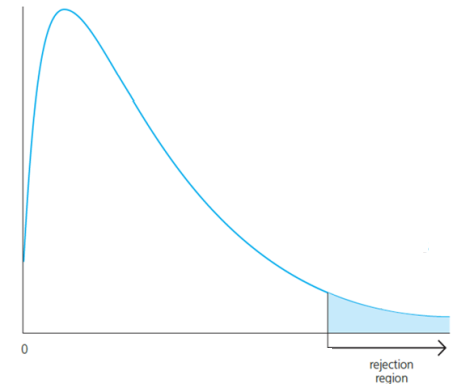
\includegraphics[scale=.3]{f_dist}
\end{figure} 
\item However, given problems with weak instruments, a rule of thumb is that if $F-score <10$, then we have a weak instrument problem 
\end{itemize}
\hyperlink{IV}{\beamerbutton{Back}}
\end{frame}










\end{document}